\documentclass[a4paper,hidelinks,12pt,twoside]{report}
\usepackage[left=3cm,right=3cm,top=3cm,bottom=3cm]{geometry} %Margins
\usepackage{pdfpages}
\usepackage[hidelinks]{hyperref}
\usepackage{listings}
\usepackage{xcolor}
\usepackage{wasysym}
\usepackage{setspace}
\usepackage{tocloft}
\usepackage[margin=1.5cm]{caption}
\usepackage{emptypage}

\usepackage{enumitem}
\usepackage{chngcntr}
\usepackage[page,toc,titletoc,title]{appendix}
\usepackage[T1]{fontenc}
\usepackage[nottoc]{tocbibind}
\usepackage[compact]{titlesec}
\titlespacing{\section}{0pt}{1ex}{0ex}
\titlespacing{\subsection}{0pt}{1ex}{0ex}
\titlespacing{\subsubsection}{0pt}{1ex}{0ex}


\counterwithin{figure}{chapter}
\counterwithin{table}{chapter}

\usepackage[utf8]{inputenc}
\usepackage{graphicx}
\usepackage{verbatim}
\usepackage{latexsym}
\def\bbbr{{\rm I\!R}} %reelle Zahlen
\def\bbbm{{\rm I\!M}}
\def\bbbn{{\rm I\!N}} %natuerliche Zahlen
\def\bbbf{{\rm I\!F}}
\def\bbbh{{\rm I\!H}}
\def\bbbk{{\rm I\!K}}
\def\bbbp{{\rm I\!P}}
\def\bbbe{{\rm I\!E}}
\def\bbbone{{\mathchoice {\rm 1\mskip-4mu l} {\rm 1\mskip-4mu l}
{\rm 1\mskip-4.5mu l} {\rm 1\mskip-5mu l}}}
\def\bbbc{{\mathchoice {\setbox0=\hbox{$\displaystyle\rm C$}\hbox{\hbox
to0pt{\kern0.4\wd0\vrule height0.9\ht0\hss}\box0}}
{\setbox0=\hbox{$\textstyle\rm C$}\hbox{\hbox
to0pt{\kern0.4\wd0\vrule height0.9\ht0\hss}\box0}}
{\setbox0=\hbox{$\scriptstyle\rm C$}\hbox{\hbox
to0pt{\kern0.4\wd0\vrule height0.9\ht0\hss}\box0}}
{\setbox0=\hbox{$\scriptscriptstyle\rm C$}\hbox{\hbox
to0pt{\kern0.4\wd0\vrule height0.9\ht0\hss}\box0}}}}
\def\bbbq{{\mathchoice {\setbox0=\hbox{$\displaystyle\rm
Q$}\hbox{\raise
0.15\ht0\hbox to0pt{\kern0.4\wd0\vrule height0.8\ht0\hss}\box0}}
{\setbox0=\hbox{$\textstyle\rm Q$}\hbox{\raise
0.15\ht0\hbox to0pt{\kern0.4\wd0\vrule height0.8\ht0\hss}\box0}}
{\setbox0=\hbox{$\scriptstyle\rm Q$}\hbox{\raise
0.15\ht0\hbox to0pt{\kern0.4\wd0\vrule height0.7\ht0\hss}\box0}}
{\setbox0=\hbox{$\scriptscriptstyle\rm Q$}\hbox{\raise
0.15\ht0\hbox to0pt{\kern0.4\wd0\vrule height0.7\ht0\hss}\box0}}}}
\def\bbbt{{\mathchoice {\setbox0=\hbox{$\displaystyle\rm
T$}\hbox{\hbox to0pt{\kern0.3\wd0\vrule height0.9\ht0\hss}\box0}}
{\setbox0=\hbox{$\textstyle\rm T$}\hbox{\hbox
to0pt{\kern0.3\wd0\vrule height0.9\ht0\hss}\box0}}
{\setbox0=\hbox{$\scriptstyle\rm T$}\hbox{\hbox
to0pt{\kern0.3\wd0\vrule height0.9\ht0\hss}\box0}}
{\setbox0=\hbox{$\scriptscriptstyle\rm T$}\hbox{\hbox
to0pt{\kern0.3\wd0\vrule height0.9\ht0\hss}\box0}}}}
\def\bbbs{{\mathchoice
{\setbox0=\hbox{$\displaystyle     \rm S$}\hbox{\raise0.5\ht0\hbox
to0pt{\kern0.35\wd0\vrule height0.45\ht0\hss}\hbox
to0pt{\kern0.55\wd0\vrule height0.5\ht0\hss}\box0}}
{\setbox0=\hbox{$\textstyle        \rm S$}\hbox{\raise0.5\ht0\hbox
to0pt{\kern0.35\wd0\vrule height0.45\ht0\hss}\hbox
to0pt{\kern0.55\wd0\vrule height0.5\ht0\hss}\box0}}
{\setbox0=\hbox{$\scriptstyle      \rm S$}\hbox{\raise0.5\ht0\hbox
to0pt{\kern0.35\wd0\vrule height0.45\ht0\hss}\raise0.05\ht0\hbox
to0pt{\kern0.5\wd0\vrule height0.45\ht0\hss}\box0}}
{\setbox0=\hbox{$\scriptscriptstyle\rm S$}\hbox{\raise0.5\ht0\hbox
to0pt{\kern0.4\wd0\vrule height0.45\ht0\hss}\raise0.05\ht0\hbox
to0pt{\kern0.55\wd0\vrule height0.45\ht0\hss}\box0}}}}
\def\bbbz{{\mathchoice {\hbox{$\mathsf\textstyle Z\kern-0.4em Z$}}
{\hbox{$\mathsf\textstyle Z\kern-0.4em Z$}}
{\hbox{$\mathsf\scriptstyle Z\kern-0.3em Z$}}
{\hbox{$\mathsf\scriptscriptstyle Z\kern-0.2em Z$}}}}
\usepackage{setspace}
\usepackage{blindtext}
\usepackage{float}

\setlength{\parskip}{\medskipamount}  % a little space before a \par
\setlength{\parindent}{0pt}	      % don't indent first lines of paragraphs
%UHEAD.STY  If this is included after \documentstyle{report}, it adds
% an underlined heading style to the LaTeX report style.
% \pagestyle{uheadings} will put underlined headings at the top
% of each page. The right page headings are the Chapter titles and
% the left page titles are supplied by \def\lefthead{text}.

% Ted Shapin, Dec. 17, 1986

\makeatletter
\def\chapapp2{Chapter}

\def\appendix{\par
 \setcounter{chapter}{0}
 \setcounter{section}{0}
 \def\chapapp2{Appendix}
 \def\@chapapp{Appendix}
 \def\thechapter{\Alph{chapter}}}

\def\ps@uheadings{\let\@mkboth\markboth
% modifications
\def\@oddhead{\protect\underline{\protect\makebox[\textwidth][l]
		{\sl\rightmark\hfill\rm\thepage}}}
\def\@oddfoot{}
\def\@evenfoot{}
\def\@evenhead{\protect\underline{\protect\makebox[\textwidth][l]
		{\rm\thepage\hfill\sl\leftmark}}}
% end of modifications
\def\chaptermark##1{\markboth {\ifnum \c@secnumdepth >\m@ne
 \chapapp2\ \thechapter. \ \fi ##1}{}}%
\def\sectionmark##1{\markright {\ifnum \c@secnumdepth >\z@
   \thesection. \ \fi ##1}}}
\makeatother
%%From: marcel@cs.caltech.edu (Marcel van der Goot)
%%Newsgroups: comp.text.tex
%%Subject: illegal modification of boxit.sty
%%Date: 28 Feb 92 01:10:02 GMT
%%Organization: California Institute of Technology (CS dept)
%%Nntp-Posting-Host: andromeda.cs.caltech.edu
%%
%%
%%Quite some time ago I posted a file boxit.sty; maybe it made it
%%to some archives, although I don't recall submitting it. It defines
%%	\begin{boxit}
%%	...
%%	\end{boxit}
%%to draw a box around `...', where the `...' can contain other
%%environments (e.g., a verbatim environment). Unfortunately, it had
%%a problem: it did not work if you used it in paragraph mode, i.e., it
%%only worked if there was an empty line in front of \begin{boxit}.
%%Luckily, that is easily corrected.
%%
%%HOWEVER, apparently someone noticed the problem, tried to correct it,
%%and then distributed this modified version. That would be fine with me,
%%except that:
%%1. There was no note in the file about this modification, it only has my
%%   name in it.
%%2. The modification is wrong: now it only works if there is *no* empty
%%   line in front of \begin{boxit}. In my opinion this bug is worse than
%%   the original one.
%%
%%In particular, the author of this modification tried to force an empty
%%line by inserting a `\\' in the definition of \Beginboxit. If you have
%%a version of boxit.sty with a `\\', please delete it. If you have my
%%old version of boxit.sty, please also delete it. Below is an improved
%%version.
%%
%%Thanks to Joe Armstrong for drawing my attention to the bug and to the
%%illegal version.
%%
%%                                          Marcel van der Goot
%% .---------------------------------------------------------------
%% | Blauw de viooltjes,                    marcel@cs.caltech.edu
%% |    Rood zijn de rozen;
%% | Een rijm kan gezet
%% |    Met plaksel en dozen.
%% |


% boxit.sty
% version: 27 Feb 1992
%
% Defines a boxit environment, which draws lines around its contents.
% Usage:
%   \begin{boxit}
%	... (text you want to be boxed, can contain other environments)
%   \end{boxit}
%
% The width of the box is the width of the contents.
% The boxit* environment behaves the same, except that the box will be
% at least as wide as a normal paragraph.
%
% The reason for writing it this way (rather than with the \boxit#1 macro
% from the TeXbook), is that now you can box verbatim text, as in
%   \begin{boxit}
%   \begin{verbatim}
%   this better come out in boxed verbatim mode ...
%   \end{verbatim}
%   \end{boxit}
%
%						Marcel van der Goot
%						marcel@cs.caltech.edu
%

\def\Beginboxit
   {\par
    \vbox\bgroup
	   \hrule
	   \hbox\bgroup
		  \vrule \kern1.2pt %
		  \vbox\bgroup\kern1.2pt
   }

\def\Endboxit{%
			      \kern1.2pt
		       \egroup
		  \kern1.2pt\vrule
		\egroup
	   \hrule
	 \egroup
   }	

\newenvironment{boxit}{\Beginboxit}{\Endboxit}
\newenvironment{boxit*}{\Beginboxit\hbox to\hsize{}}{\Endboxit}
\pagestyle{empty}

\setlength{\parskip}{2ex plus 0.5ex minus 0.2ex}
\setlength{\parindent}{0pt}

\makeatletter  %to avoid error messages generated by "\@". Makes Latex treat "@" like a letter

\linespread{1.5}
\def\submitdate#1{\gdef\@submitdate{#1}}
\def\supervisor#1{\gdef\@supervisor{#1}}
\def\cosupervisor#1{\gdef\@cosupervisor{#1}}

\def\maketitle{
  % Title
  \begin{titlepage}{
    \vspace*{2\baselineskip} %Empty Lines
    {\fontsize{17.28}{16.8}\selectfont Master's Thesis on Sound and Music Computing}\\
     {\fontsize{14}{16.8}\selectfont Universitat Pompeu Fabra}\\
    \rm
    \vspace*{3\baselineskip} %Empty Lines
     \bf \fontsize{24.88}{17.5}\selectfont  \@title \par
  }
  \vskip 0.3in
  \par
  {\fontsize{14}{27}\selectfont  \@author}

  \vskip 0.20in
  \fontsize{14}{16.8}\selectfont \textbf{Supervisor:}   \@supervisor \\
  %\fontsize{14}{16.8}\selectfont \textbf{Co-Supervisor:}  \@cosupervisor \\
   \vspace*{3\baselineskip} %Empty Lines
    \fontsize{14}{27}\selectfont  \@submitdate \\
    \vspace{ 0.7in}
    
\includegraphics[width=8cm]{Figures/LogoPompeuFabra}\\[.5cm]
  \vfil
  \end{titlepage}
}

\def\titlepage{
  \newpage
  \centering
  \linespread{1.5}
  \normalsize
  \vbox to \vsize\bgroup\vbox to 9in\bgroup
}
\def\endtitlepage{
  \par
  \kern 0pt
  \egroup
  \vss
  \egroup
}

\def\abstract{
  \begin{center}{
    \large\bf Abstract}
  \end{center}
  \small
  %\def\baselinestretch{1.5}
  \linespread{1.5}
  \normalsize
}
\def\endabstract{
  \par
   \cleardoublepage
}

\newenvironment{acknowledgement}{
  \clearpage
  \begin{center}{
    \large \bf Acknowledgement}
  \end{center}
  \small
  \linespread{1.5}
  \normalsize
}{\clearpage}
\def\endacknowledgement{
  \par
    \cleardoublepage
}

\newenvironment{dedication}{
\pagenumbering{roman}%
  \clearpage
  \small
  \linespread{1.5}
  \normalsize
}{\clearpage}
\def\enddedication{
  \par
  \cleardoublepage
}

\def\preface{
    
    \pagestyle{plain}
    \doublespacing
     \setcounter{tocdepth}{2}
    \tableofcontents
    \cleardoublepage 
    \listoffigures
    \cleardoublepage
    \listoftables
    \cleardoublepage 
}

\def\body{

    \clearpage    
    \pagestyle{uheadings}
    \pagenumbering{arabic}
    \singlespacing  
    \setlength{\cftbeforesecskip}{10pt}

    \pagestyle{plain}
    \clearpage
    \pagestyle{uheadings}
    
}

\makeatother  %to avoid error messages generated by "\@". Makes Latex treat "@" like a letter

\newcommand{\titlelinespacing}{\renewcommand{\baselinestretch}{2.0} \normalsize}
\newcommand{\normallinespacing}{\renewcommand{\baselinestretch}{1.5} \normalsize}
\newcommand{\mediumlinespacing}{\renewcommand{\baselinestretch}{1.2} \normalsize}
\newcommand{\narrowlinespacing}{\renewcommand{\baselinestretch}{1.0} \normalsize}

\newtheorem{definition}{Definition}[chapter]
\newtheorem{theorem}{Theorem}[chapter]
\cftsetindents{section}{0.2in}{0.4in}
\cftsetindents{subsection}{0.4in}{0.5in}
\cftsetindents{paragraph}{0in}{0.5in}


\begin{document}

\newgeometry{left=2cm,right=2cm} %Only for the title new margins

%Title parameters
\title{Computational modelling of expressive music performance in hexaphonic guitar}
\author{Marc Siquier Peñafort}
\submitdate{September 2017}
\supervisor{Sergio Giraldo Méndez}
%\cosupervisor{Rafael Ramírez}

\maketitle
\vfill
\vspace*{\fill}
\hrule
Copyright: \copyright  2017 <Marc Siquier Peñafort>. This is an open-access document distributed
under the terms of the Creative Commons Attribution-ShareAlike License 4.0 International (CC BY-SA 4.0). Please see license conditions at \url{https://creativecommons.org}.
\maketitle
\cleardoublepage
\restoregeometry
\sloppy

\begin{dedication}
\textit{"We learned more from a three minute record\\ than we ever learned in school"}

Springsteen, Bruce. "No Surrender". \textit{Born in the U.S.A.}
\newpage
\end{dedication}

%\addcontentsline{toc}{chapter}{Acknowledgement}

\begin{acknowledgement}
The present work was carried out at Music and Machine Learning Department of the Music Technology Group at Universitat Pompeu Fabra, Barcelona, Spain.

First of all, I want to thank the supervisor of this thesis Sergio Giraldo, whose previous work, advise and ideas have been fundamentals to this project.

... 

Last  but  not  least, I  am  very grateful to  my  family for their unconditional support and encouragement over these years. Many thanks.

\newpage
\end{acknowledgement}
\begin{abstract}

% In this Master's Thesis, we present a work on a machine learning approach to automatically generate expressive performances from non expressive music scores of polyphonic guitar. We are going to treat guitar as an hexaphonic instrument and capture each string separately in order to obtain a better transcription. Features extracted from the scores and the corresponding audio recordings performed by a professional guitarist are going to be used to train computational models for guitar modelling and predicting performance actions such as onset deviation, duration deviation or energy ratio.

Computational modelling of expressive music performance has been widely studied in the past. While previous work in this area has been mainly focused on classical piano music, there has been very little work on guitar music, and such work has focused on monophonic guitar playing. In this work, we present a machine learning approach to automatically generate expressive performances from non expressive music scores for polyphonic guitar. We treated guitar as an hexaphonic instrument, obtaining a polyphonic transcription of performed musical pieces. 
Features were extracted from the scores and performance actions were calculated from the deviations of the score and the performance. Machine learning techniques were used to train computational models to predict the aforementioned performance actions. Qualitative and quantitative evaluations of the models and the predicted pieces were performed. 

\newpage
\cleardoublepage

\begin{center}{
    \large\bf Resum}
  \end{center}
 %\todo[inline]{Traduir abstract al català}
 
% En aquesta tesi de màster treballarem en la generació automàtica de models d'expressivitat a partir de partitures musicals no expresives per a guitarra polifònica utilitzant aprenentatge automàtic. Tractarem la guitar com un instrument hexafònic i capturarem cada corda per separat, amb la finalitat d'obtenir una millor transcripció. Les característiques extretes a partir de les partitures i les corresponents gravacions d'àudio realitzades per un guitarrista professional seran utilitzades per entrenar models computacionals per a modelar i predir les petites accions expressives o ornamentacions de la melodia com deviació en onsets, en duració o en energia.

El modelatge computacional de interpretacions expressives de peces músicals ha estat àmpliament estudiat en el passat. Tot i que el treball previ en aquesta àrea s'ha centrat principalment en la música clàssica per piano, hi ha hagut molt poc treball sobre música per guitarra i aquest s'ha centrat en la guitarra monofònica. En aquest treball, utilitzem aprenentatge automàtic per generar automàticament interpretacions expressives a partir de partitures de música no expressiva per a guitarra polifònica. Tractem la guitarra com a un instrument hexafònic, obtenint una transcripció polifònica de les peces musicals interpretades.
A partir de les partitures s'han extret diverses característiques i s'han calculat accions interpretatives a partir de les desviacions entre la partitura i la interpretació del músic. Diverses tècniques d'aprenentatge automàtic s'han utilitzat per entrenar models computacionals i predir les accions interpretatives esmentades anteriorment. Finamlent s'han realitzat avaluacions qualitatives i quantitatives dels models i les peces predites.

\end{abstract}



\preface
\body

%project

\normallinespacing

\chapter{Introduction}


\label{chap:introduction}
Music is a very important part of the life of most people. Depending on our mood or moment in the day or lives, music can be understood in very different ways. In some moments we understand music as a simple distraction, a soundtrack to our daily tasks without paying much attention to it. In other moments, when we consciously listen to music we can be very touched and excited by it. This engaging part of music is largely due to the human component added to the performance. Instead of reading a score, musicians play the music on their way, by changing (unconsciously) a lot of "parameters" of it such as intensity, velocity, volume or articulation of each note. 

The study of music expressive performance from a computational point of view consists of characterizing this deviations that a musician introduces in a score. In this work we are going to focus on modelling guitar scores and performances. In this chapter we discuss the motivation of this master's thesis, the main objectives and we explain briefly the structure of this report.

\section{Motivation}
Most studies about guitar modelling are focused on monophonic performances, the main goal of this master thesis is to enhance the system proposed by Giraldo~\cite{Giraldo2016} in order to compute expressive performance models for polyphonic guitar. The main objective of this thesis will be to define a set a features that are able to extend previous work on monophonic guitar performances to polyphonic performances. Those features need to represent the different nuances in time, duration or volume that the guitarist performs, the added ornamentation present in the temporal or \textit{horizontal} axis (as a monophonic melody), but also should represent the \textit{vertical} axis representing the simultaneity between notes.

Understanding this little nuances and ornamentation that professional players perform when reading and performing a score could help less trained musicians to improve their playing. This models could also be used by music annotation software in order to generate expressive performances from scores composed by users, and get a better idea on how the score would be performed by a professional guitar player instead a straight forward score to midi conversion.

\section{Objectives}
The aim of this work is to study computationally the little nuances or \textit{Performance Actions} that musicians do when performing a score, focusing only in polyphonic guitar performances considering both horizontal or melodic axis and vertical or harmonic axis.

The specific objectives are as follows:

\begin{itemize}[noitemsep]
\item To create a database of hexaphonic recordings played by a guitarist and the corresponding scores.
\item To automatically transcribe the audio of the hexaphonic recordings into a machine-readable format (MIDI).
\item To create code libraries to extract descriptors from the score which allow us to characterize the notes vertically and horizontally.
\item To create code libraries which allow us to align and compare the transcribed recordings to the score in order to extract performance actions.
\item To provide a few manually corrected performance to score alignments.
\item To generate different models that try to predict performance actions (onset deviation and energy ration) by using Machine Learning techniques.
\item To analyse which descriptors influence more the accuracy of these models, so to say, which descriptors represent more the behaviour of the musician.
\end{itemize}

\section{Structure of the report}
The rest of this thesis is organized as follows: in Chapter~\ref{chap:sota}, we present some related work in expressive music performance modelling specially focused on polyphonic music. In Chapter~\ref{chap:materials}, the materials used in this work are described. In Chapter~\ref{chap:methods}, we present the proposed methodology. In Chapter~\ref{chap:results}, the evaluation measures and results are presented. We conclude with a brief discussion and provide suggestions for future improvements in Chapter~\ref{chap:discussion}. \\
In order to complement this thesis we present 3 Appendices: Appendix~\ref{app:dataset} documenting the dataset used for this work, Appendix~\ref{app:code} documenting the developed code and Appendix~\ref{app:survey} gathering all responses to the On-line Survey.
\cleardoublepage


\normallinespacing
\chapter{State of the art}
\label{chap:sota}
In this section we will review the state of the art in music expression, giving an
overview of the past and present research in the field. Specifically focusing in polyphonic music expression modelling where machine learning has been used to predict some kind of performance actions.

The state of the art of this work can be divided in two parts: first, in section~\ref{sec:muexpmod}, we review the works related to music expressive performances modelling. Finally, in section~\ref{sec:autohexaguit} we provide examples of works that try to automatically transcribe guitar, focusing on those treating guitar as an hexaphonic instrument transcribing each string separately. 

\section{Music expression modelling}
\label{sec:muexpmod}

Performance Actions (PAs) can be defined as musical resources used by musicians to add expression when performing a musical piece, which consist of little nuances (variations in timing, pitch, and energy) that are not indicated in a score. In the same context, ornamentation can be considered as an expressive musical resource used to embellish and add expression to a melody. This PAs are what make music expressive and differentiate it from a robotic performance, this little nuances, done mostly unconsciously, are part of our human nature and it's what make us feel and enjoy a musical performance as something unique. This uniqueness of a performance based on the variation in timing, dynamics, timbre and pitch was first proposed by Juslin~\cite{Juslin2001}. Ramirez and Hazan~\cite{Ramirez2006} add the punctuation that those little variations should be clearly distinguishable for listeners.

In the past, music expression has been mostly studied in the context of classical music and most research focus on studying timing deviations (onset nuances), dynamics (energy) and vibrato (pitch nuances). Some studies try to obtain rules to represent that performance actions by hand from music experts. There are several expert-based systems studying this field from different perspectives. The KTH group developed a set of several rules~(\cite{Friberg2009}) for predicting tempo, energy and pitch variations included in a system called \textit{Director Musices}. Parts of the rule system were implemented in other programs (see for instance the work by Sundberg~\cite{Sundberg2003} that tries to use rules to predict \textit{Inter Onset intervals} or Bresin~\cite{Bresin2000} who try to generate macro rules for predicting PAs).

\begin{table}[ht!]
\centering
  \caption{State of the art few expert-based methods table review.}
  \label{tab:sota_experts}
  \begin{tabular}{  l l l l }
    \hline
	Author & System & Instrument \\ \hline
    KTH & Director Musices & General\\
    Sundberg & Inter-Onset & Piano\\
    Bresin & DM mapped to emotions & General\\
    \hline
  \end{tabular}

\end{table}


On the other hand, machine-learning-based systems try to obtain the set of rules (expressive models) directly from the music performance by trying to directly measure the PAs applied by the performer. This PAs are computed by measuring deviations of the expressive performance (done by a professional performer) with respect to a neutral or robotic data (such as strict MIDI representations of the score). For an overview of theses methods see the review by Goebl~\cite{Goebl2005}, from where we can see that most of the proposed expressive music systems are in classical music, and most of these systems are based on piano performances. Those kind of machine-learning systems started arising since simple synthesiser keyboards or digital pianos were used to capture expressive performances. Those devices allowed accurate timing and loudness data to be sent via MIDI (Musical Instrument Digital Interface) to a computer.

In order to obtain these expressive performance models, several types of machine learning algorithms have been used, Bresin~\cite{Bresin1998} tries to model piano performances using Artificial Neural Networks (ANN) by trying to learn automatically the Director musices rules stated by KTH group. Camurri~\cite{Camurri2000} also applied ANN in order to obtain music expression for flute performances. He also developed a 2D representation of the expression space using non-linear projections in order to be able to choose between different emotions and their middle points.

Widmer~\cite{Widmer2003a} (also in~\cite{Widmer2003}) used rule-based learning and meta-learning algorithms in order to cluster piano performances. He developed a new rule discovery algorithm named PLCG (Partition+Learn+Cluster+Generalize) that can find simple, robust partial rules models (sets of classification rules) in complex data where it is difficult or impossible to find models that completely account for all the data. PLCG is an ensemble learning method that learns multiple models via some standard rule learning algorithm, and then combines these into one final rule set via clustering, generalization, and heuristic rule selection. He also uses this algorithm and discovered rules to predict multi-level timing and dynamics~\cite{Widmer2003}.

Grindlay~\cite{Grindlay2006} utilizes Hidden Markov Models in order to extract Performance Actions from performances from both students pianists and professional pianists in order to model different performances. He uses HMM in order to predict time variations from a non-expressive score. In his work Miranda~\cite{Miranda2010} uses a generative performance system based on genetic algorithms in order to predict those time variations. 

Contrary to classical music scores, performance annotations (e.g. ornaments, dynamics and articulations ) are seldom indicated in popular music scores, and it is up to the performer to include them based on his/her musical background. Therefore, in popular music it may not always be possible to characterize ornaments with the archetypal classical music conventions (e.g. trills and \textit{appoggiaturas}). 

Several approaches have been proposed to generate expressive performances not in piano-classical music. Arcos~\cite{Arcos1998} proposed a system that generates jazz solo saxophone expressive performances, based on case-based reasoning. In his work, several recordings of a tenor sax playing different Jazz ballads were made. These recordings were analysed to extract information related to several expressive parameters. This set of parameters and the scores constitute the set of cases of a case-based system. From this set of cases, the system infers a set of possible expressive transformations for a given new phrase applying similarity criteria, based on background musical knowledge, between this new phrase and the set of cases.

Gratchen~\cite{Grachten2006} also applies case-based reasoning to generate models for ornamentation and tempo variations for jazz saxophone music. He's system automatically performs melodic and expressive analysis, and when a new musical performance must be tempo-transformed, it uses the most similar example tempo-transformation to infer the changes of expressiveness that are necessary to make the result sound natural.

Ramirez~\cite{Ramirez2006} generates a tool in order to both generating and explaining expressive music performances of monophonic Jazz melodies for saxophone. The tool consists of three components a melodic transcription component which extracts a set of acoustic features from monophonic recordings, a machine learning component which induce both an expressive transformation model and a set of expressive performance rules from the extracted acoustic features, and a melody synthesis component which generates expressive monophonic output (MIDI or audio) from inexpressive melody descriptions using the induced expressive transformation model.

Puiggros~\cite{Puiggros2006} try to generate automatic characterization of ornamentation from bassoon recordings in order to generate expressive synthesis. His work addresses the characterization of expressive bassoon ornaments by analysing audio recordings played by a professional bassoonist. This characterization is then used to generate expressive ornaments from symbolic representations by means of Machine Learning

Previous work on guitar expressive performance modelling has mainly been done by Sergio Giraldo~\cite{Giraldo2016} who use machine learning techniques to model ornamentation and PAs in monophonic jazz guitar performances according to the characteristics of the notes' context. Features extracted from scores and their corresponding audio recordings performed by a professional guitarist are used to train computational models for predicting melody ornamentation. Several machine learning techniques were explored to induce regression models for timing, onset, and dynamics (i.e. note duration and energy) transformations, and an ornamentation model for classifying notes as ornamented or non-ornamented.

Bantula~\cite{bantula2016} models expressive performance for a jazz ensemble of guitar and piano. The interesting part of this work is the polyphonic treatment done to the piano, extracting features for chords played such as \textit{density, weight} or \textit{range}. Kirke et al~\cite{KirkeAlexisMiranda2013} models polyphonic piano recordings with generative experiments that show that multiple polyphonic expressive actions can be found in human expressive performances. 

In table~\ref{tab:sota_ml} we can see an overview of authors, methods and instruments where music expression modelling using machine learning was applied.

\begin{table}[ht!]
\centering
  \caption[State of the art machine learning methods table review.]{State of the art machine learning methods table review. Non exhaustive table.}
  \label{tab:sota_ml}
  \begin{tabular}{  l l l l }
    \hline
	Author & Method & Instrument & Mono/Poly \\ \hline
    Arcos & Case based reasoning & Saxophone & monophonic\\
    Bantula & Several methods & Jazz ensemble & polyphonic \\
    Bresin & $ANN$ & Piano & monophonic\\
    Camurri & $ANN$ & Flute & monophonic\\
    Giraldo & Several methods & Guitar & monophonic \\
    Gratchen & Case based reasoning & Saxophone & monophonic \\
    Grindlay & $HMM$ & Piano & monophonic\\
    Kirke & Generative models & Piano & polyphonic \\
    Miranda & Genetic Algorithms & Piano & monophonic\\
    Puiggros & Several methods & Bassoon & monophonic \\
    Ramirez & Several methods & Saxophone & monophonic \\
    Widmer & Rule-based meta-learning & Piano & monophonic\\
 
    
    \hline
  \end{tabular}

\end{table}


\section{Automatic hexaphonic guitar transcription}
\label{sec:autohexaguit}
When we think about music transcription we usually think about a music expert hearing over and over a musical piece and writing it down to a traditional score notation. Defined by Klapuri~\cite{Klapuri2004} music transcription is defined as \textit{"the process of analysing an acoustic musical signal so as to write down the musical parameters of the sounds that occur in it"}. So, the traditional main goal of music transcription is to represent music as detailed as possible, so it can be accurately reproduced afterwards. 

Nowadays, we also think about music transcription as the way to convert acoustic music signal to a machine readable format, such as MIDI, XML or piano-roll representation in order to be analysed and processed produce a notation reflecting the most relevant information about the musical events within it, as an output. 	

One of the main difficulties when facing automatic music transcription is given by the number of voices a musical signal has, or the number of sound sources that are present in it. Limiting the problem to one single source (as it is in our case) makes us confront with another problem: monophonic and polyphonic sources. The main problem of this task is now pitch detection. 

While in the monophonic case is practically considered to be a solved problem within the state of the art techniques (Klapuri 2004~\cite{Klapuri2004}). However, polyphonic case is really far from being solved specially for multi-instrumental contexts. The main problem of polyphonic transcription is multiple fundamental frequency estimation and tacking and tracking, which is a very difficult task when two or more concurrent sounds contain partials that share some frequencies. Knowing in advance the different sources eases a bit the task~\cite{argenti2011}. There are some works with good results in multiple fundamental frequency detection by Klapuri~\cite{Klapuri2006} who tries to estimate multiple fundamental frequencies calculating the salience, or strength, of a F0 candidate as a weighted sum of the amplitudes of its harmonic partials. This F0 salience spectrum is found by optimization using generated training material.

In our case, working with guitar music, transcription process is a difficult task due to the polyphonic nature of the sound it emits.
As said before, limiting the player to just produce a monophonic sound eases the process as thre exist very good and state of the art approaches such as the autocorrelation method, Yin or spectral peak picking, among others.

However, the main goal of this project is to extend a monophonic system to a polyphonic one, so polyphonic transcription is one of the main tasks of it. Reviewing the literature we find a few approaches for transcribing polyphonic guitar music. Fiss \& Kwasinksi propose a system for automatic guitar audio transcription in real time~\cite{Fiss2011}. This approach is based on the STFT (Short Time Fourier Transform) to compute the spectrogram used to extract information about the peak locations. Afterwards they try to correct the note detector by taking into account the probability of each note being being produced among the six strings of the guitar, and thus, avoiding the ambiguity of polyphonic guitar.
 
As stated above, avoiding polyphony makes the transcription task much easier. So, the idea of capturing and transcribing separately each string makes a lot of sense. Asking the musician to think about the whole song but just playing the notes on one string would probably be very difficult as well as non musical at all. 

Solving this little problem, O'Grady \& Rickard~\cite{OGrady2009} proposed a solution based on the Roland GK-3 divided pick-up~\cite{gk3} which captures separately each string in order to be processed with a guitar synthesizer and create really strange and creative sounds with it. For the transcription of that six different signals they used Non-Negative Matrix Factorization (NMF) where a matrix V is factorized into two matrices W and H, with the property that all three matrices have no negative elements. In this case, for one string $W_{string}$ contained the magnitude spectrum of all possible notes played on that string, resulting $H_{string}$ as an activation matrix indicating the position in time in which each note was played.


\cleardoublepage
\chapter{Materials}
\label{chap:materials}
For this project, we have used several materials which can be divided into 3 categories: hardware, software and data.

\section*{Hardware}
\begin{itemize}[noitemsep]
\item Roland GK-3: the hexaphonic recordings were done using this special divided pick-up
\item Breakout Box: this adaptor box was needed in order to convert the output from the GK-3 to 6 standard Jack connectors.
\item PC: Intel Core i5-6600 CPU @ 3.30GHz, 16.0GB RAM
\end{itemize}

\section*{Software}
\begin{itemize}[noitemsep]
\item ProTools HD 10: it was used in order to generate a mix the 6 strings channels. It also was used to synthesize midi both from the transcribed performances and from the predicted performance.
\item MuseScore 2: the scores in XML format for the performances were written using MuseScore.
\item Python: the code for transcribing guitar performances was developed by using Python.
\item Essentia: we used a few algorithms (in order to transcribe guitar) from this open-source C++ library for audio analysis and audio-based music information retrieval.
\item Matlab: the code for extracting the features from the performance and from the scores was developed by using Matlab.
\item MIDI Toolbox: the MidiToolBox Library developed by Toivianinen and Ereola (implemented in Matlab) allowed us to process easily MIDI data.
\item Weka Data Mining Software: it was used to train and test different machine learning models, to implement feature selection and to analyze the results.
\end{itemize}

\section*{Data}
For this work we used a set of three recordings done by Helena Bantula for her Master's thesis consisting of one recording of \textit{Darn that dream} by Jimmy Van Heusen and Eddie De.Lange and two recordings of \textit{Suite en la} by Manuel M. Ponce.

Their corresponging scores where written using Musescore and extracted as XML files.

\cleardoublepage
\chapter{Methodology}
\label{chap:methods}
Four separate stages of this thesis can be defined: data acquisition (guitar recording), transcription, feature extraction and models computation. Expressive hexaphonic guitar recordings will be done using the Roland GK-3 divided pick-up, which is able to separate sound from each string~\cite{Angulo2016}. The main output of this first stage will be a new dataset consisting of hexaphonic recordings recorded by a professional guitar player with different performance actions of the performance depending on a given mood. \\
After this step, transcription of each individual string will be computed applying non-negative matrix factorization~\cite{OGrady2009}. After doing a score alignment with the original score and the transcription of the expressive guitar performance, feature extraction needs to be done.\\
Feature extraction will be performed following an approach in which each note is characterized by its \textit{nominal}, \textit{neighbouring}, and \textit{contextual} properties.  Here is where the most of the research in this thesis will take place:  checking for literature in expressive piano modelling, combining it with previously mentioned features of monophonic expressive guitar modelling,... \\
Several machine learning and feature selection algorithms will be applied to predict those performance actions (timing, pitch, energy,...) and ornaments introduced by the musician when performing a musical piece.


\section{Data acquisition}
In order to obtain hexaphonic recordings and get each string nicely separated we used the Roland GK-3 divided pickup that is easily attached to any steel-stringed electric guitar and acts as a sound transduction device. It is able to separate very good the sound from each string and delivers accurate performance data. \\
However, the output of this pickup consists of a 13 pin DIN cable that allows to connect the guitar to guitar synthesizers such as Roland's popular GR-55 and at the same time to fed electrically the pickup. So, in order to be able to record each string separately we need to adapt the pickup output so the sound of each string can be inputted to the computer through an independent input chanel of an audio interface.\\
To do this, a Breakout Box circuit was built by I.Angulo~\cite{Angulo2016} for his master's thesis last year so we reused it. The final box has an input for the 13 pin DIN cable and 6 separate Jack connector cables are outputted, one for each string. Also, two batteries are needed inside the box in order to fed the pickup.



\section{Hexaphonic guitar transcription}


\section{Feature extraction}
\begin{table}[ht!]
\centering
  \caption[Chord description.] {Chord description. A list of chords definitions.  The numbers on the Intervals column indicate the index of the notes belonging to the chord, (zero indexed, in 12 semitones).}
  \label{tab:chord_extensions}
  \begin{tabular}{  l  c  l }
    \hline
    Chord type & Intervals & Example (C as root) \\ \hline
    M (major) & 0 4 7 & C E G \\
    m (minor) & 0 3 7 & C E$\flat$ G \\
    2 (sus2) & 0 2 7 & C D G \\
	sus (sus4) & 0 5 7 & C F G \\
    dim & 0 3 6 &  C E$\flat$ G$\flat$\\
    + (Aug) & 0 4 8 & C E G$\sharp$ \\
	Maj7 & 0 4 7 11 & C E G B \\
	6 (6th) & 0 4 7 9 & C E G A \\
	m7 & 0 3 7 10 & C E$\flat$ G B$\flat$ \\
	m6 & 0 3 7 9 & C E$\flat$ G A \\
	mMaj7 & 0 3 7 11 & C E$\flat$ G B \\
    m7$\flat$5 & 0 3 6 1 0& C E$\flat$ G$\flat$ B$\flat$ \\
    dim7 & 0 3 6 9 & C E$\flat$ G$\flat$ A \\
	7 (7th) & 0 4 7 10 & C E G B$\flat$ \\
	7\#5 & 0 4 8 10 & C E G$\sharp$ B$\flat$ \\
	7$\flat$5 & 0 4 6 10 & C E G$\flat$ B$\flat$ \\
	7sus & 0 5 7 10 & C F G B$\flat$ \\
	Maj9 & 0 2 4 7 11 & C D E G B \\
	69 (6/9) & 0 2 4 7 9 & C D E G A \\
	m9 & 0 2 3 7 9 & C D E$\flat$ G A \\
	9 (9th) & 0 2 4 7 10 & C D E G B$\flat$ \\
	7$\flat$9 & 0 1 4 7 10 & C D$\flat$ E G B$\flat$ \\
	7\#9 & 0 3 4 7 10 & C D$\sharp$ E G B$\flat$ \\
	13 (13th) & 0 2 4 7 9 10 & C D E G A B$\flat$ \\
	7$\flat$9$\flat$13 & 0 1 4 7 8 10 & C D$\flat$ E G A$\flat$ B$\flat$ \\
	7alt & 0 1 3 4 6 8 10 & C D$\flat$ E$\flat$ E G$\flat$ A$\flat$ B$\flat$ \\
    \hline
  \end{tabular}

\end{table}


\subsection{Note Descriptors}
\begin{table}
\centering
  \caption[Complete list of descriptors extracted from music scores.]{Complete list of descriptors extracted from music scores.}
  \label{tab:note_descriptors}
   \makebox[\textwidth][c]{
  \footnotesize
  \begin{tabular}{l l c c c p{2.5cm} }
    \hline 
    Code & Descriptor & Abbreviation & Units & Formula & Range \\ \hline
    
	7 & Duration & $ds_n$ & Seconds & $ds_0$ & [0,+$\infty$] \\
    2 & Duration & $db_n$ & Beats & $db_0$ & [0,+$\infty$] \\
 	6 & Onset & $ons_n$ & Seconds & $os_0$ & [0,+$\infty$] \\
 	1 & Onset & $onb_n$ & Beats & $ob_0$ & [0,+$\infty$] \\
 	15 & Onset in bar & $obm_n$ & Beats & $ob_0\%bpb$ & [0,+bpb] \\
 	4 & Pitch & $p_n$ & Semitones & $p_0$ & [1,127] \\
 	16 & Chroma & $ch_n$ & Semitones & $p_0\%12$ & [0,11] \\
 	5 & Energy & $v_n$ & MIDI vel & $v_0$ & [1,127] \\ 
    3 & String & $str_n$ & String num & $channel_0$ & [1,6] \\\hline 
    
	10 & Prev. duration & $pds_n$ & Seconds & $ds_{-1}$ & [0,+$\infty$] \\
 	9 & Prev. duration & $pdb_n$ & Beats & $db_{-1}$ & [0,+$\infty$] \\
    12 & Next duration & $nds_n$ & Seconds & $ds_1$ & [0,+$\infty$] \\
    11 & Next duration & $ndb_n$ & Beats & $db_1$ & [0,+$\infty$] \\
    18 & Prev. interval & $pint_n$ & Semitones & $p_{-1}-p_0$ & [-60,60] \\
 	19 & Next interval & $nint_n$ & Semitones & $p_1-p_0$ & [-60,60] \\
 	13 & Prev. inter-onset dist. & $piod_n$ & Seconds & $os_0-os_{-1}$ & [0,+$\infty$] \\
 	14 & Next. inter-onset dist. & $piod_n$ & Seconds & $os_1-os_0$ & [0,+$\infty$] \\
 	28 & Narmour & $nar1_n$ & Label & $nar(p_{-1},p_0,p_1)$ & [P, D, R, ID]\\
    29 & & $nar2_n$ &  & $nar(p_{-2},p_{-1},p_0)$ & [VR, IR, VP, IP] \\
	30 & & $nar3_n$ & & $nar(p_0,p_1,p_2)$ & [dyadic, monadic, none] \\
    33 & Is a Chord & $ich_n$ & Boolean & $isChord_0$ & \{true, false\} \\
    34 & Is a Pedal & $pdl_n$ & Boolean & $pdl_0$ & \{true, false\} \\
    17 & Simultaneous notes & $sim_n$ & Number & $simult_0$ & [0,+$\infty$] \\ \hline
    
    8 & Measure & $m_n$ & Bars & $m_0$ & [0,+$\infty$] \\
    31 & Tempo & $t_n$ & Bpm & $t_0$ & [30,260] \\
    20 & Key & $k_n$ & Semitones & $k_0$ & [-6,6] \\
 	35 & Mode & $mod_n$ & Label & $mod_0$ & \{major, minor\} \\
 	23 & Chord root & $chr_n$ & Semitones & $chr_0$ & [0,11] \\
    24 & Chord type & $cht_n$ & Label & $cht_0$  & \{+, 6, 7, 7\#11, 7\#5, 7\#9, 7alt, 7$\flat$5, 7$\flat$9, Maj7, dim, dim7, m, m6, m7, m7$\flat$5, major\} \\
    21 & Note to key & $n2k_n$ & Semitones & $ch_0-k_0$ & [0,11] \\
	25 & Note to chord & $n2ch_n$ & Semitones & $ch_0-chr_0$ & [0,11] \\
 	26 & Is chord note & $ichn_n$ & Boolean & $isChNote$ & \{true, false\} \\
 	27 & Metrical strength & $mtr_n$ & Label & $metStr_0$ & \{Very strong, Strong, Weak, Very weak\} \\
 	32 & Phrase & $ph_n$ & Label & $phrase_0$ & \{initial, middle, final\} \\
 

    \hline

  \end{tabular}
  }
\end{table}


\subsection{Performance to score alignment}


\begin{figure}
  \caption{\textit{Darn that dream} 8 beats manually corrected}
  \centering
    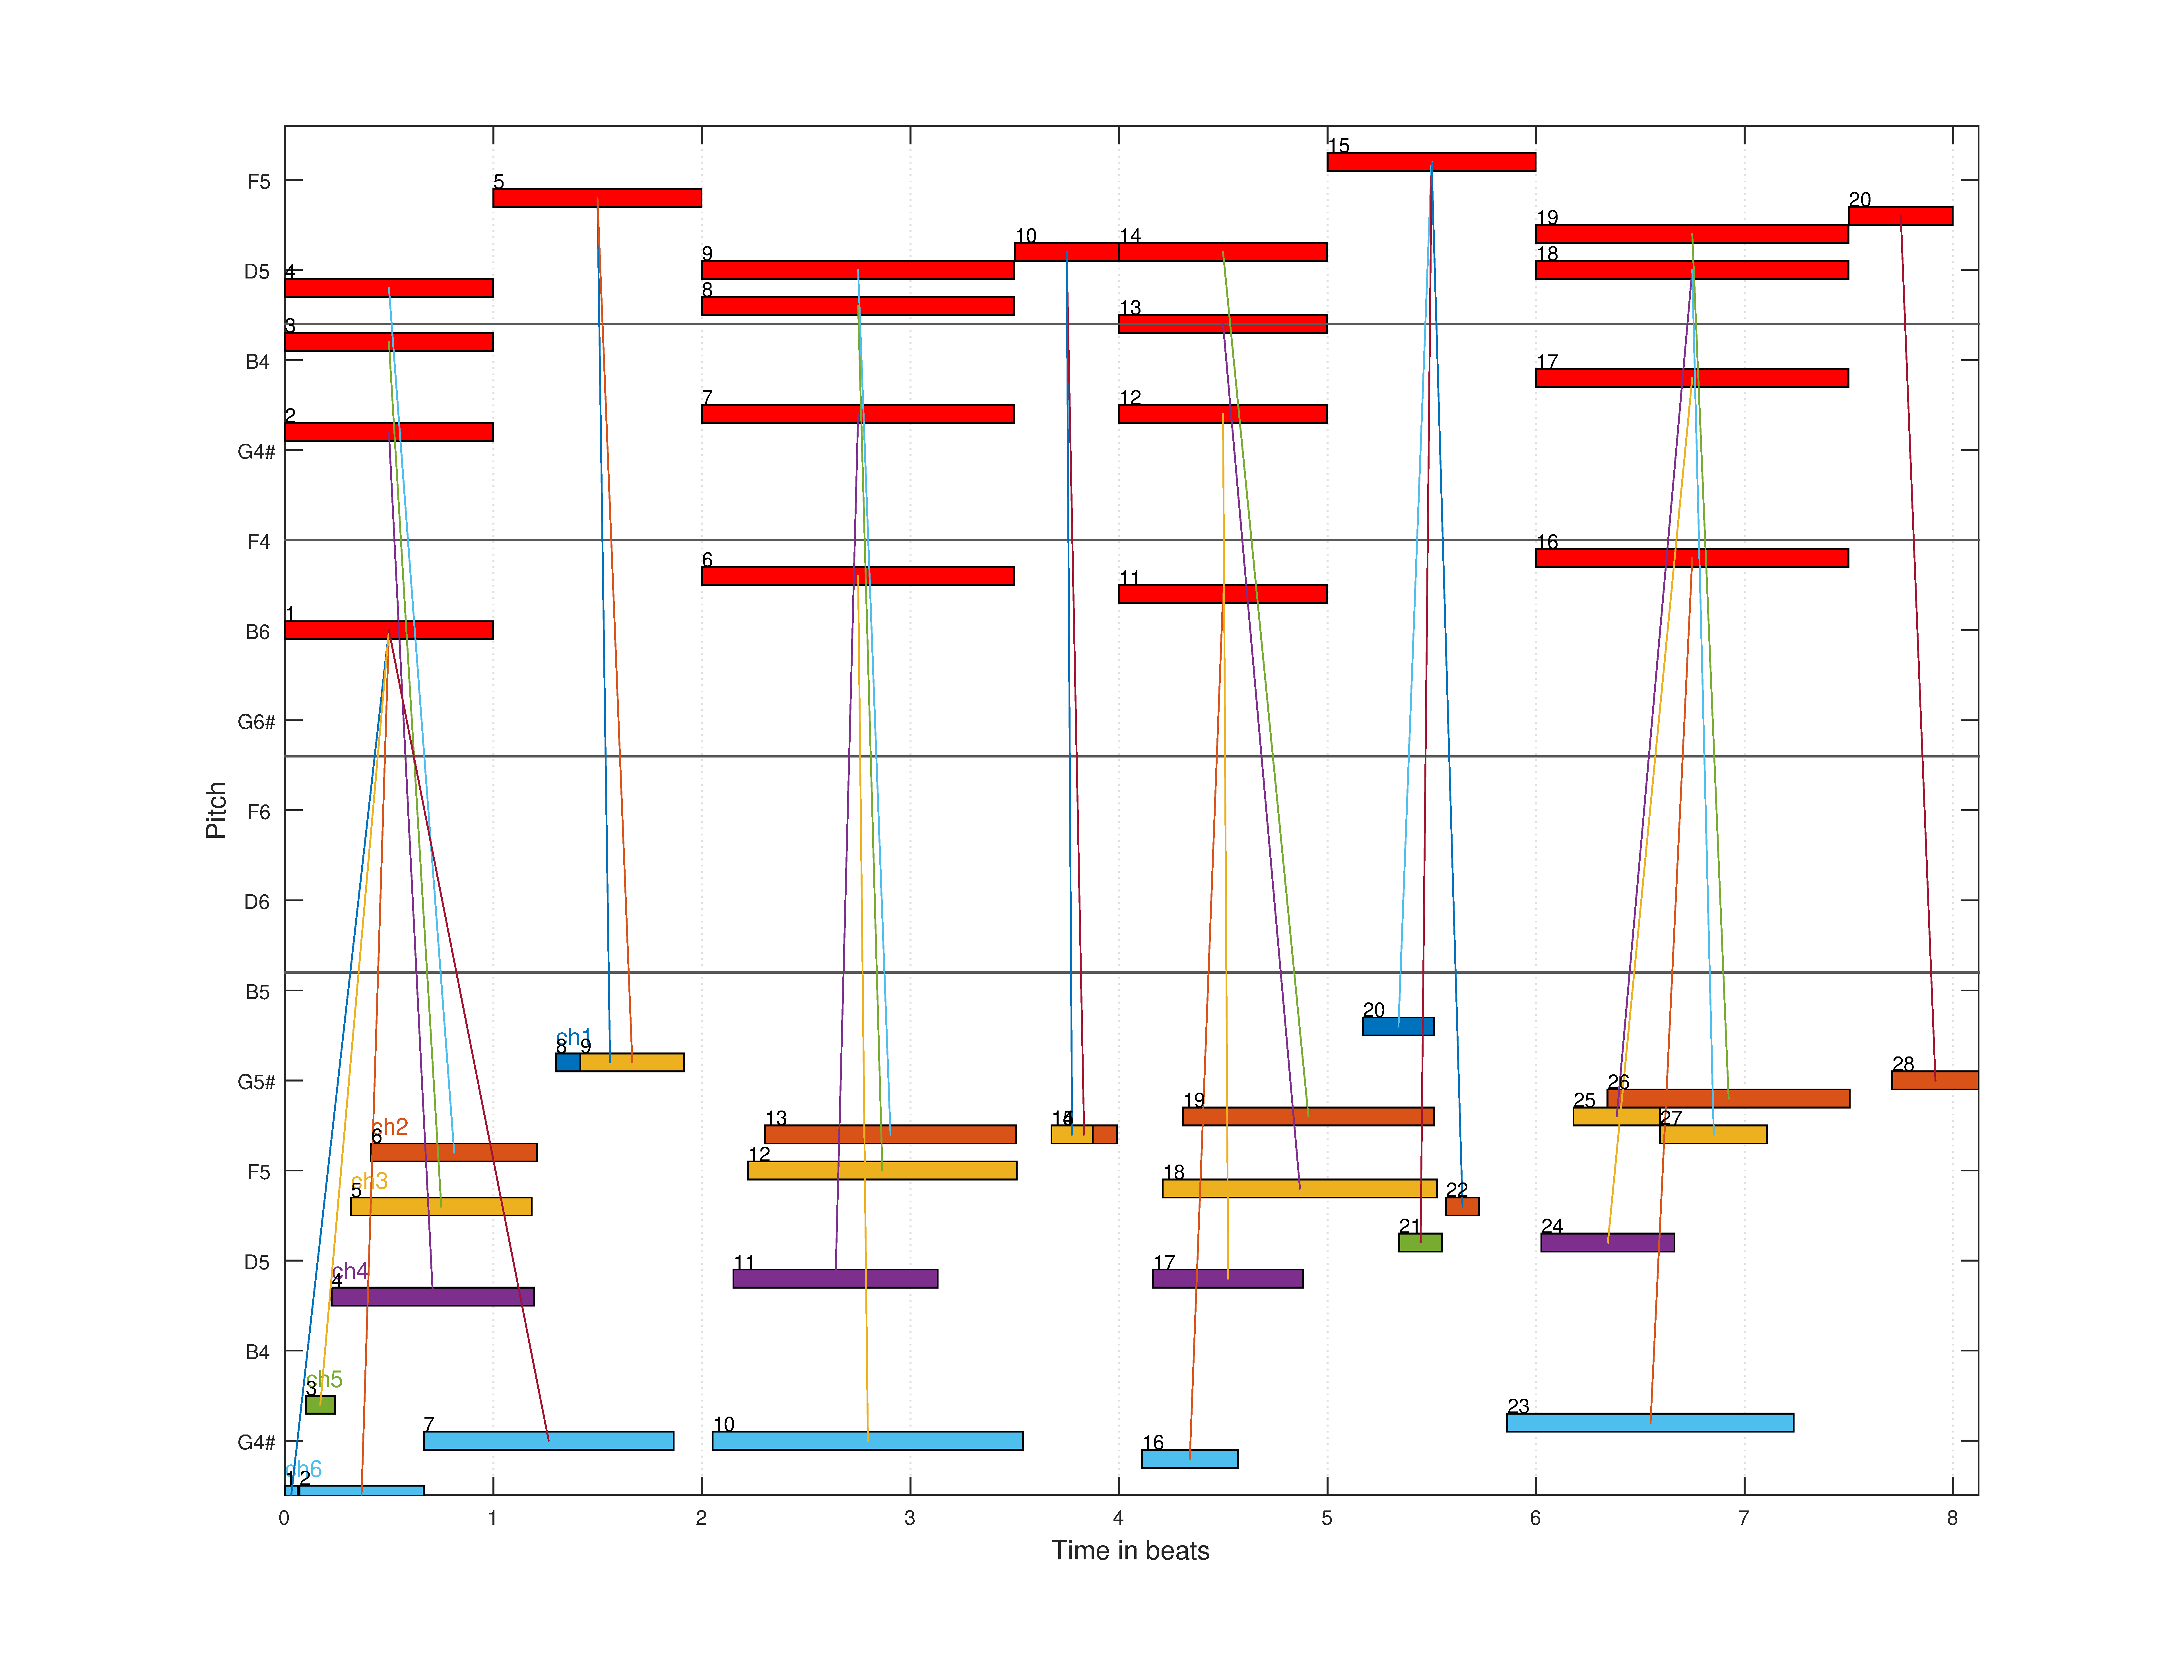
\includegraphics[width=0.7\textwidth]{Figures/Darn_8b_corrected.pdf}
\end{figure}
\subsection{Performance actions}
\section{Machine Learning modelling}
\cleardoublepage


\chapter{Results}
\label{chap:results}
\section{Feature Selection}
\section{Evaluation Measures}
\section{Evaluation Results}

\newpage
\begin{table}
\centering
\caption[Results comparing different ML models (10 fold Cross-Validation)]{Results comparing different ML models (10 fold Cross-Validation). All datasets correspond to the three datasets merged into one. Shown values correspond to Correlation Coefficients.}
\label{tab:results_ml_cv}
\footnotesize
\begin{tabular} {lcccHcccH}
\\ \hline
\multirow{2}{3cm}{Dataset (feature)} & D.Tree & $k_1NN$ & $k_2NN$ & $k_4NN$ & $k_8NN$ & SVM & ANN & L.Reg \\ 
& cv/train & cv/train & cv/ train & cv/train & cv/train & cv/train & cv/train & cv/train\\\hline

'Darn (energy)' & 0.37/0.53 & 0.18/1 &  0.27/0.78 & 0.27/0.64 &  0.28/0.52 &  0.37/0.55 & 0.26/0.98 & 0.35/0.58 \\
'Darn (onset)' & 0.70/0.87 & 0.35/1 &  0.42/0.83 & 0.48/0.75 & 0.52/0.69 & 0.57/0.68 & 0.47/0.99 & 0.56/0.71  \\
'Suite (energy)' & 0.35/0.59 & 0.24/1 & 0.31/0.77 & 0.33/0.64 & 0.32/0.53 &  0.23/0.38 &  0.17/0.70 & 0.26/0.43 \\
'Suite (onset)' & 0.77/0.88 & 0.28/1 & 0.35/0.80 & 0.37/0.70 & 0.33/0.53 & 0.30/0.40 & 0.29/0.79 & 0.30/0.44 \\
'Suite2 (energy)' & 0.32/0.70 & 0.21/1 & 0.24/0.77 & 0.19/0.59 & 0.17/0.45 & 0.19/0.31 & 0.18/0.66 & 0.19/0.39 \\
'Suite2 (onset)' & 0.83/0.92 & 0.43/1 & 0.48/0.85 & 0.45/0.74 & 0.51/0.85 & 0.44/0.52 & 0.40/0.78 & 0.44/0.55 \\ \hline

'All (energy)' & 0.35/0.51 & 0.22/1 & 0.26/0.78 & 0.27/0.64 & 0.27/0.51 & 0.21/0.33 & 0.23/0.63 & 0.25/0.38 \\
'All (onset)' & 0.67/0.77 & 0.30/1 & 0.36/0.81 & 0.42/0.69 & 0.42/0.60 & 0.39/0.45 & 0.29/0.67 & 0.40/0.47 \\ 
'All (energy)'$_{5 features}$ & 0.41/0.50 & 0.30/1 & 0.37/0.80 & 0.39/0.67 & 0.37/0.57 & 0.14/0.21 & 0.14/0.36 & 0.16/0.23 \\
'All (onset)'$_{5 features}$ & 0.69/0.72 & 0.38/1 & 0.61/0.82 & 0.65/0.79 & 0.65/0.75 & 0.30/0.31 & 0.44/0.43 & 0.31/0.32 \\
'All (energy)'$_{best subset}$ & 0.41/0.51 & 0.30/1 & 0.37/0.79 & 0.38/0.66  & 0.37/0.57  & 0.16/0.21 & 0.15/039 & 0.15/0.23 \\
'All (onset)'$_{best subset}$ & 0.69/0.73 & 0.37/1 & 0.58/0.82 & 0.62/0.78 & 0.64/0.73 & 0.30/0.32 & 0.48/0.48 &  0.31\\

\hline
\end{tabular} 
\footnotesize

\end{table}

\begin{table}
\centering
\caption[Results comparing different ML models (Train/Test)]{Results comparing different ML models (Train/Test). In this table 66\% of the Dataset has been used as Train and 33\% as Test. Notes has been randomly selected. Shown values correspond to Correlation Coefficients.}
\label{tab:results_ml_tt}
\footnotesize

\begin{tabular} {lcccccccc}
\\ \hline
Dataset (feature) & D.Tree& $k_1NN$ & $k_2NN$ & $k_4NN$ & $k_8NN$ & SVM & ANN & L.Reg \\ \hline
'Darn (energy\_rat)' & 0.44 & 0.14  & 0.21  & 0.23  & 0.31  & 0.32  & 0.34  & 0.35 \\
'Darn (onset\_dev)' & 0.58 & 0.41  & 0.49  & 0.44  & 0.41  & 0.56  & 0.39  & 0.51 \\
'Suite (energy\_rat)' & 0.33 & 0.30  & 0.27  & 0.27  & 0.31  & 0.19  & 0.21  & 0.23 \\
'Suite (onset\_dev)' & 0.67 & 0.32  & 0.43  & 0.44  & 0.42  & 0.35  & 0.39  & 0.39 \\
'Suite2 (energy\_rat)' & 0.31 & 0.21  & 0.17  & 0.15  & 0.06  & 0.11  & 0.23  & 0.12 \\
'Suite2 (onset\_dev)' & 0.79 & 0.37  & 0.51  & 0.48  & 0.56  & 0.45  & 0.44  & 0.49 \\

\hline
\end{tabular}


\footnotesize

\end{table}

\begin{table}
\centering

\footnotesize
\begin{tabular} {llccHHcc}
\\ \hline

%% & \multicolumn{2}{c}{$k_1NN$}

 \multirow{2}{1cm}{Train} &  \multirow{2}{1cm}{Test} & \multicolumn{2}{c}{D.Tree} & & & \multicolumn{2}{c}{ANN}\\ 
 &  & energy & onset & energy & onset & energy & onset	 \\ \hline
'Darn' & 'Suite' & 0.013 & 0.156 & 0.110 & 0.069 & 0.047 & 0.008 \\
'Darn' & 'Suite2' & 0.091 & 0.183 & 0.018 & 0.177 & 0.033 & 0.075 \\
'Suite' & 'Darn' & 0.017 & 0.140 & 0.333  & 0.11 & 0.107 & 0.032 \\
'Suite' & 'Suite2' &  0.324 & 0.392 & 0.215 & 0.338 & 0.148 & 0.253 \\
'Suite2' & 'Darn' & 0.043 & 0.099 & 0.061 & 0.1672 & 0.079 & 0.027 \\
'Suite2' & 'Suite' & 0.240 &  0.384 & 0.2316 & 0.349 & 0.190 & 0.227 \\
\hline
\end{tabular} 
\footnotesize

\caption[Results mixing songs for Train/Test]{Results mixing songs for Train/Test. Whole song Datasets have been used in order to train or test. Shown values correspond to Correlation Coefficients.}
\label{tab:results_mixed}

\end{table}


\cleardoublepage


\chapter{Discussion}
\label{chap:discussion}
\section{Discussion}

\section{Conclusions}

\section{Future Work}

\cleardoublepage



% appendices come here
\bibliographystyle{naturemag}
\bibliography{bibliography}
\cleardoublepage

\begin{appendices}
\cleardoublepage
\chapter{Dataset Documentation}
\label{app:dataset}


\cleardoublepage

\chapter{Code Documentation} 
\label{app:code}
\cleardoublepage

\chapter{Online Survey Responses}
\label{app:survey}

\begin{figure}
\caption{On-line survey instructions.}
\label{fig_app:survey_instructions}
\centering
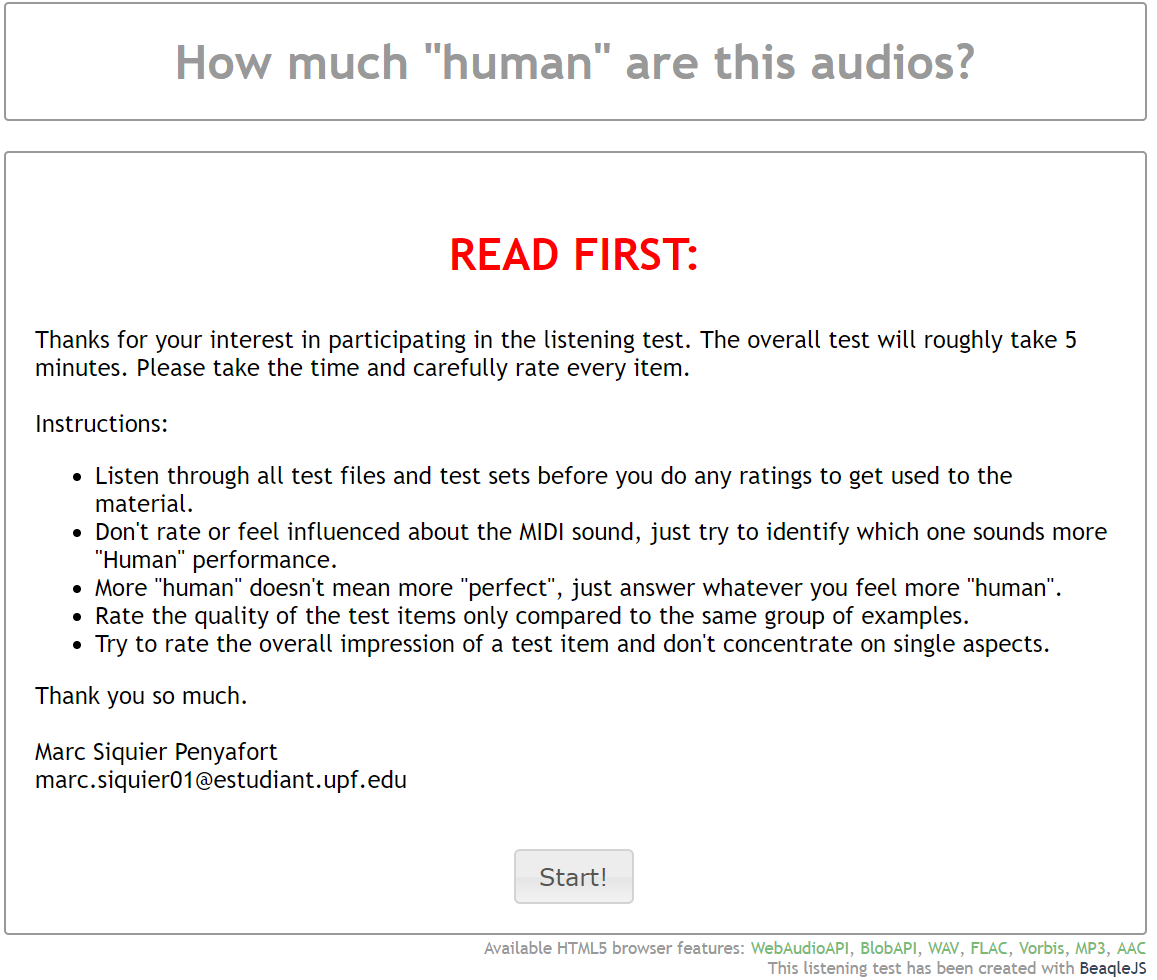
\includegraphics[width=0.8\textwidth]{Figures/survey_instructions.PNG}
\end{figure}

\begin{figure}
\caption{On-line survey example of a Test set.}
\label{fig_app:survey_test}
\centering
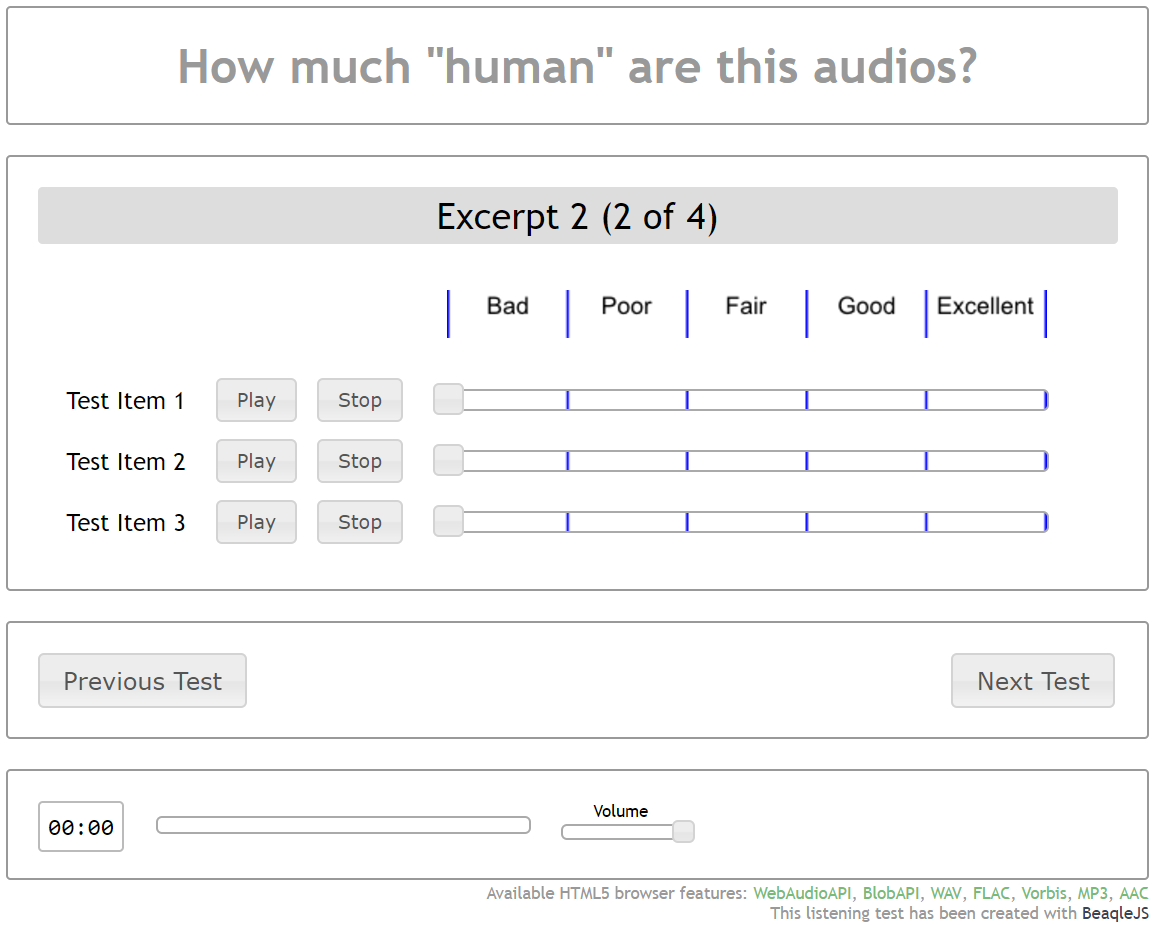
\includegraphics[width=0.8\textwidth]{Figures/survey_test.PNG}
\end{figure}

\begin{table}[ht!]
\centering
  \caption[Full table results of the on-line survey.]{Full table results of the on-line survey.}
  \label{tab:survey_results}
  \footnotesize
\begin{tabular}{l|ccc|ccc|ccc|ccc}

\hline
\multicolumn{1}{c}{\multirow{2}{*}{}} & \multicolumn{3}{c}{intro1} & \multicolumn{3}{c}{intro2} & \multicolumn{3}{c}{middle}  & \multicolumn{3}{c}{end} \\ 
\multicolumn{1}{c}{}                      & \multicolumn{1}{c}{Perf} & \multicolumn{1}{c}{Pred} & \multicolumn{1}{c}{Score} & \multicolumn{1}{c}{Perf} & \multicolumn{1}{c}{Pred} & \multicolumn{1}{c}{Score} & \multicolumn{1}{c}{Perf} & \multicolumn{1}{c}{Pred} & \multicolumn{1}{c}{Score} & \multicolumn{1}{c}{Perf} & \multicolumn{1}{c}{Pred} & \multicolumn{1}{c}{Score} \\ \hline
1 & 20 & 51 & 43 & 63 & 43 & 83 & 40 & 26 & 75 & 75 & 34 & 40 \\ 
2 & 31 & 29 & 76 & 73 & 33 & 91 & 13 & 29 & 52 & 13 & 25 & 88 \\ 
3 & 61 & 39 & 62 & 48 & 35 & 69 & 57 & 30 & 61 & 45 & 47 & 62 \\
4 & 49 & 49 & 55 & 63 & 43 & 83 & 29 & 66 & 76 & 45 & 67 & 78 \\
5 & 46 & 37 & 50 & 45 & 47 & 81 & 70 & 50 & 76 & 40 & 37 & 80 \\ 
6 & 35 & 69 & 26 & 70 & 65 & 50 & 39 & 70 & 50 & 32 & 91 & 68 \\
7 & 50 & 71 & 49 & 50 & 50 & 50 & 68 & 54 & 87 & 35 & 68 & 69 \\
8 & 33 & 72 & 50 & 70 & 71 & 29 & 66 & 68 & 47 & 90 & 47 & 68 \\
9 & 40 & 19 & 53 & 49 & 61 & 72 & 49 & 30 & 49 & 20 & 9 & 52 \\
10 & 31 & 12 & 50 & 66 & 46 & 96 & 51 & 63 & 67 & 44 & 66 & 88 \\ 
11 & 57 & 30 & 65 & 42 & 31 & 62 & 38 & 32 & 69 & 45 & 34 & 61 \\ \hline                  
\end{tabular}

\end{table}

\begin{figure}
\caption{Results of the on-line survey with performance, predicted and straight score synthesized midis.}
\label{fig_app:survey}
\centering
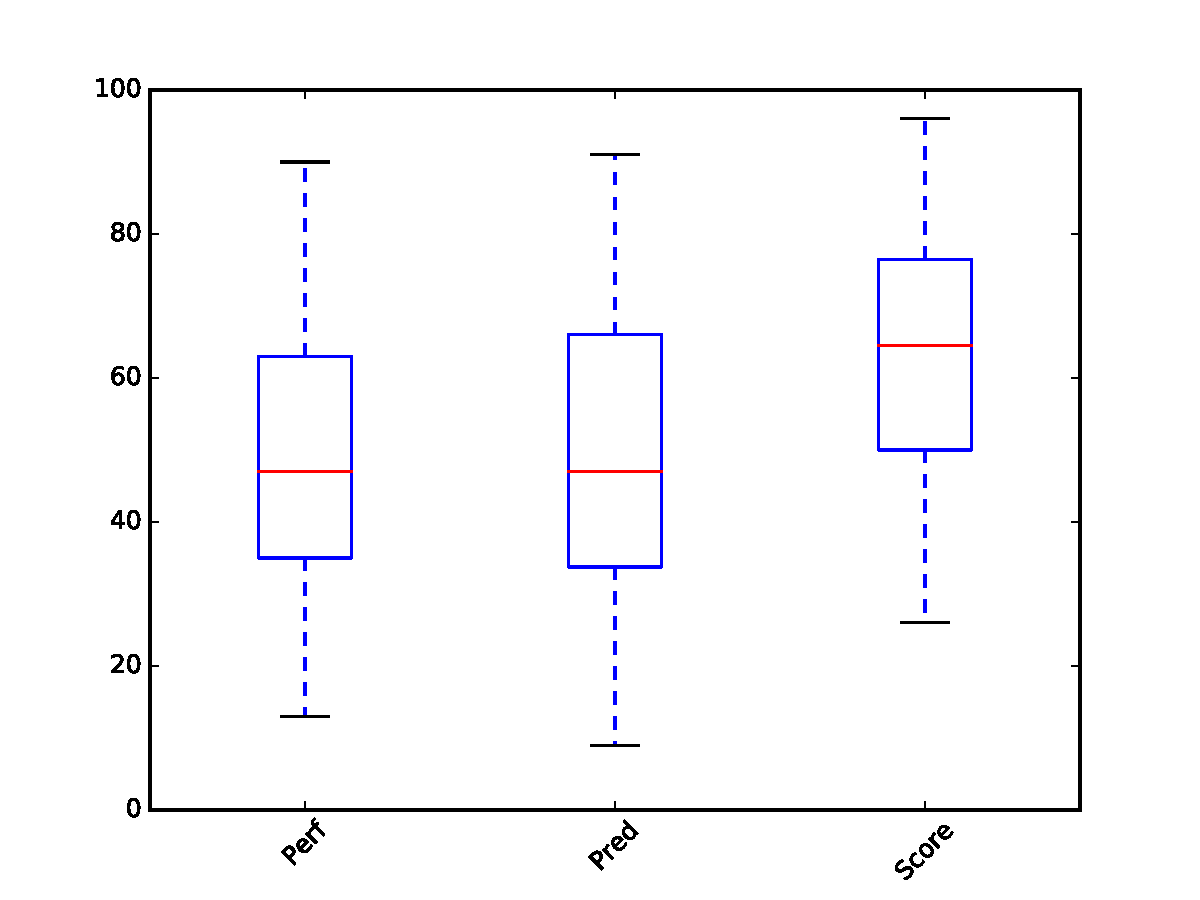
\includegraphics[width=0.8\textwidth]{Figures/survey.pdf}
\end{figure}

\begin{figure}
\caption{Results per test of the on-line survey with performance, predicted and straight score synthesized midis.}
\label{fig_app:survey_test}
\centering
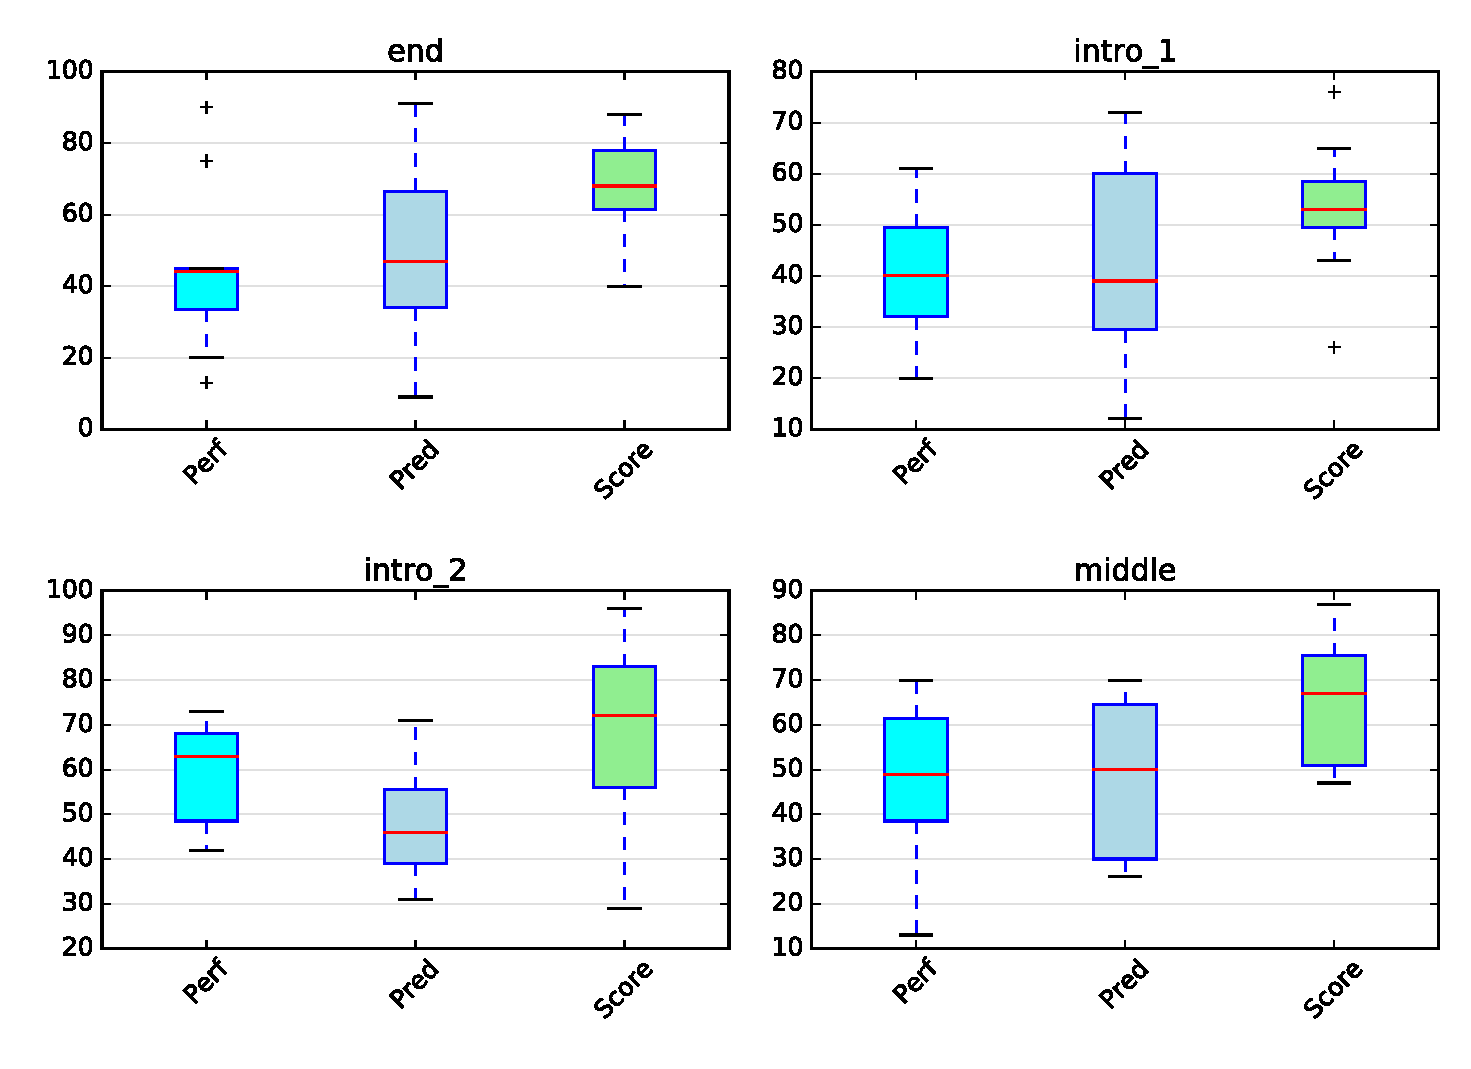
\includegraphics[width=0.8\textwidth]{Figures/survey_tests.pdf}
\end{figure}

\begin{figure}
\caption{Runtime for each test of the on-line survey.}
\label{fig_app:survey_runtime}
\centering
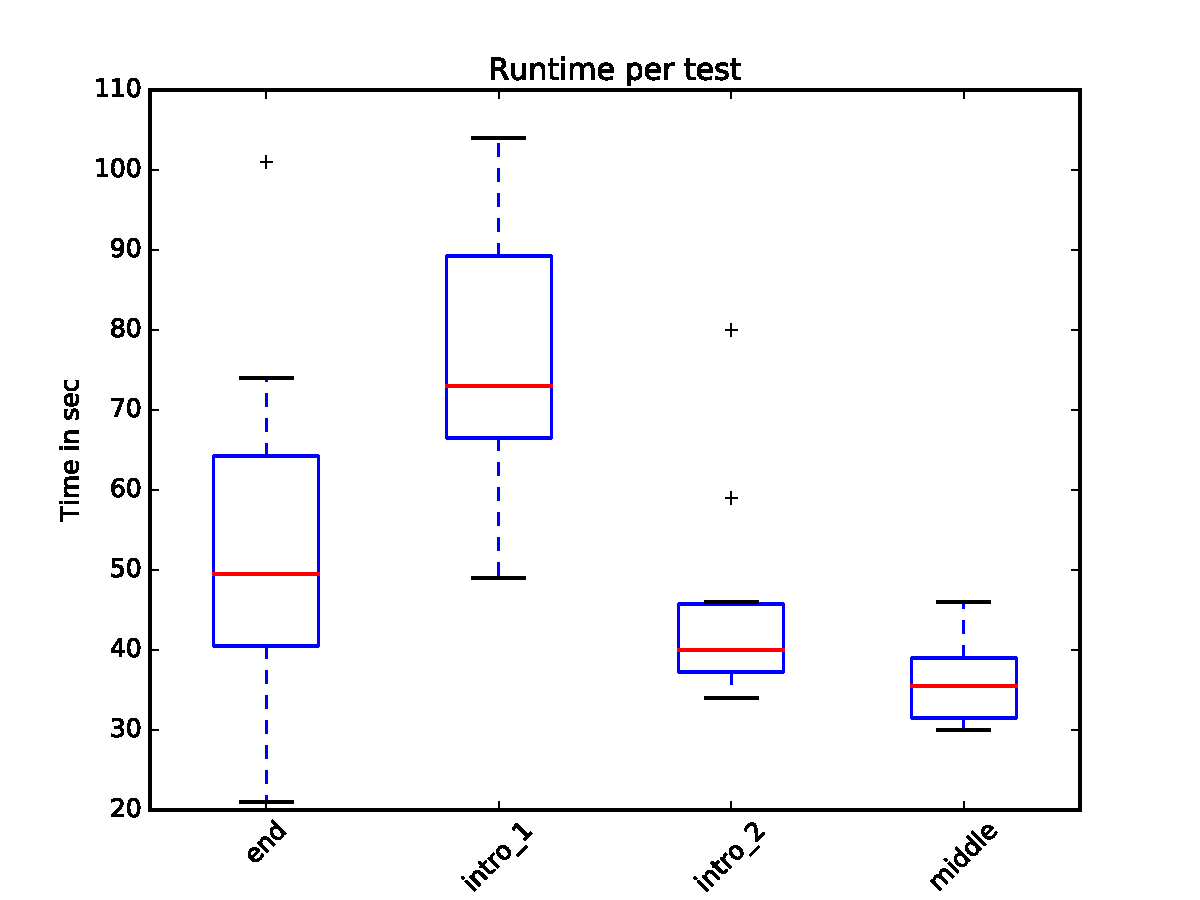
\includegraphics[width=0.8\textwidth]{Figures/survey_runtime.pdf}
\end{figure}

\cleardoublepage

\end{appendices}



\end{document}